
\documentclass[11pt,compress,t,notes=noshow, xcolor=table]{beamer}
\usepackage[]{graphicx}\usepackage[]{color}
% maxwidth is the original width if it is less than linewidth
% otherwise use linewidth (to make sure the graphics do not exceed the margin)
\makeatletter
\def\maxwidth{ %
  \ifdim\Gin@nat@width>\linewidth
    \linewidth
  \else
    \Gin@nat@width
  \fi
}
\makeatother

\definecolor{fgcolor}{rgb}{0.345, 0.345, 0.345}
\newcommand{\hlnum}[1]{\textcolor[rgb]{0.686,0.059,0.569}{#1}}%
\newcommand{\hlstr}[1]{\textcolor[rgb]{0.192,0.494,0.8}{#1}}%
\newcommand{\hlcom}[1]{\textcolor[rgb]{0.678,0.584,0.686}{\textit{#1}}}%
\newcommand{\hlopt}[1]{\textcolor[rgb]{0,0,0}{#1}}%
\newcommand{\hlstd}[1]{\textcolor[rgb]{0.345,0.345,0.345}{#1}}%
\newcommand{\hlkwa}[1]{\textcolor[rgb]{0.161,0.373,0.58}{\textbf{#1}}}%
\newcommand{\hlkwb}[1]{\textcolor[rgb]{0.69,0.353,0.396}{#1}}%
\newcommand{\hlkwc}[1]{\textcolor[rgb]{0.333,0.667,0.333}{#1}}%
\newcommand{\hlkwd}[1]{\textcolor[rgb]{0.737,0.353,0.396}{\textbf{#1}}}%
\let\hlipl\hlkwb

\usepackage{framed}
\makeatletter
\newenvironment{kframe}{%
 \def\at@end@of@kframe{}%
 \ifinner\ifhmode%
  \def\at@end@of@kframe{\end{minipage}}%
  \begin{minipage}{\columnwidth}%
 \fi\fi%
 \def\FrameCommand##1{\hskip\@totalleftmargin \hskip-\fboxsep
 \colorbox{shadecolor}{##1}\hskip-\fboxsep
     % There is no \\@totalrightmargin, so:
     \hskip-\linewidth \hskip-\@totalleftmargin \hskip\columnwidth}%
 \MakeFramed {\advance\hsize-\width
   \@totalleftmargin\z@ \linewidth\hsize
   \@setminipage}}%
 {\par\unskip\endMakeFramed%
 \at@end@of@kframe}
\makeatother

\definecolor{shadecolor}{rgb}{.97, .97, .97}
\definecolor{messagecolor}{rgb}{0, 0, 0}
\definecolor{warningcolor}{rgb}{1, 0, 1}
\definecolor{errorcolor}{rgb}{1, 0, 0}
\newenvironment{knitrout}{}{} % an empty environment to be redefined in TeX

\usepackage{alltt}
\newcommand{\SweaveOpts}[1]{}  % do not interfere with LaTeX
\newcommand{\SweaveInput}[1]{} % because they are not real TeX commands
\newcommand{\Sexpr}[1]{}       % will only be parsed by R
\newcommand{\xmark}{\ding{55}}%


\usepackage[english]{babel}
\usepackage[utf8]{inputenc}

\usepackage{dsfont}
\usepackage{verbatim}
\usepackage{amsmath}
\usepackage{amsfonts}
\usepackage{amssymb}
\usepackage{bm}
\usepackage{csquotes}
\usepackage{multirow}
\usepackage{longtable}
\usepackage{booktabs}
\usepackage{enumerate}
\usepackage[absolute,overlay]{textpos}
\usepackage{psfrag}
\usepackage{algorithm}
\usepackage{algpseudocode}
\usepackage{eqnarray}
\usepackage{arydshln}
\usepackage{tabularx}
\usepackage{placeins}
\usepackage{tikz}
\usepackage{setspace}
\usepackage{colortbl}
\usepackage{mathtools}
\usepackage{wrapfig}
\usepackage{bm}
\usepackage{amsmath}
\usepackage{pifont}
\usepackage{xcolor} %colored math symbols

\usetikzlibrary{shapes,arrows,automata,positioning,calc,chains,trees, shadows}
\tikzset{
  %Define standard arrow tip
  >=stealth',
  %Define style for boxes
  punkt/.style={
    rectangle,
    rounded corners,
    draw=black, very thick,
    text width=6.5em,
    minimum height=2em,
    text centered},
  % Define arrow style
  pil/.style={
    ->,
    thick,
    shorten <=2pt,
    shorten >=2pt,}
}

\usepackage{subfig}

% Defines macros and environments
\usepackage{../../style/lmu-lecture}


\let\code=\texttt
\let\proglang=\textsf

\setkeys{Gin}{width=0.9\textwidth}

\setbeamertemplate{frametitle}{\expandafter\uppercase\expandafter\insertframetitle}

\usepackage{bbm}
% basic latex stuff
\newcommand{\pkg}[1]{{\fontseries{b}\selectfont #1}} %fontstyle for R packages
\newcommand{\lz}{\vspace{0.5cm}} %vertical space
\newcommand{\dlz}{\vspace{1cm}} %double vertical space
\newcommand{\oneliner}[1] % Oneliner for important statements
{\begin{block}{}\begin{center}\begin{Large}#1\end{Large}\end{center}\end{block}}


%new environments
\newenvironment{vbframe}  %frame with breaks and verbatim
{
 \begin{frame}[containsverbatim,allowframebreaks]
}
{
\end{frame}
}

\newenvironment{vframe}  %frame with verbatim without breaks (to avoid numbering one slided frames)
{
 \begin{frame}[containsverbatim]
}
{
\end{frame}
}

\newenvironment{blocki}[1]   % itemize block
{
 \begin{block}{#1}\begin{itemize}
}
{
\end{itemize}\end{block}
}

\newenvironment{fragileframe}[2]{  %fragile frame with framebreaks
\begin{frame}[allowframebreaks, fragile, environment = fragileframe]
\frametitle{#1}
#2}
{\end{frame}}


\newcommand{\myframe}[2]{  %short for frame with framebreaks
\begin{frame}[allowframebreaks]
\frametitle{#1}
#2
\end{frame}}

\newcommand{\remark}[1]{
  \textbf{Remark:} #1
}


\newenvironment{deleteframe}
{
\begingroup
\usebackgroundtemplate{
\includegraphics[width=\paperwidth,height=\paperheight]{../style/color/red.png}}
 \begin{frame}
}
{
\end{frame}
\endgroup
}
\newenvironment{simplifyframe}
{
\begingroup
\usebackgroundtemplate{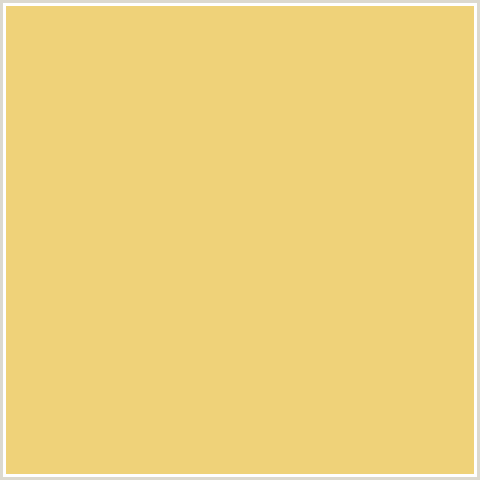
\includegraphics[width=\paperwidth,height=\paperheight]{../style/color/yellow.png}}
 \begin{frame}
}
{
\end{frame}
\endgroup
}\newenvironment{draftframe}
{
\begingroup
\usebackgroundtemplate{
\includegraphics[width=\paperwidth,height=\paperheight]{../style/color/green.jpg}}
 \begin{frame}
}
{
\end{frame}
\endgroup
}
% https://tex.stackexchange.com/a/261480: textcolor that works in mathmode
\makeatletter
\renewcommand*{\@textcolor}[3]{%
  \protect\leavevmode
  \begingroup
    \color#1{#2}#3%
  \endgroup
}
\makeatother


\input{../../latex-math/basic-math}
\input{../../latex-math/basic-ml}
\input{../../latex-math/ml-nn}

\begin{document}

\lecturechapter{6}{Advanced Components of CNNs}
\lecture{Deeplearning}
%%%%%%%%%%%%%%%%%%%%%%%%%%%%%%%%%%%%%%%%%%%%%%%%%%%%%%%%%%%%%%%%%%

\begin{frame}
\frametitle{Lecture outline}
\tableofcontents
\end{frame}
%%%%%%%%%%%%%%%%%%%%%%%%%%%%%%%%%%%%%%%%%%%%%%%%%%%%%%%%%%%%%

\begin{vbframe}{Important Types of Convolutions}


\vspace*{0.2cm}

In this chapter, we discuss further advanced components of CNNs: 

    \begin{enumerate}
    \item Inception Modules 
    \item Skip Connections 
    \item Global Average Pooling
    \end{enumerate}
\end{vbframe}

%%%%%%%%%%%%%%%%%%%%%%%%%%%%%%%%%%%%%%%%%%%%%%%%%%%%%%%%%%%%%%%%%%

\section{Inception Modules}

\begin{vbframe}{Inception modules}
    \begin{itemize}
        \item Problem setting: how do we choose the kernel size in each layer? 
        \item This is often an arbitrary decision.
        \item Solution: offer the model kernels of different sizes in each layer through which it can propagate information and let it decide, which one to use to which extent.
        \item Side-effect: massive parameter reduction allowing for deeper architectures.
        \item First proposed in \textit{Szegedy et. al , 2014}.
    \end{itemize}
\framebreak
  \begin{figure}
    \centering
      \scalebox{0.75}{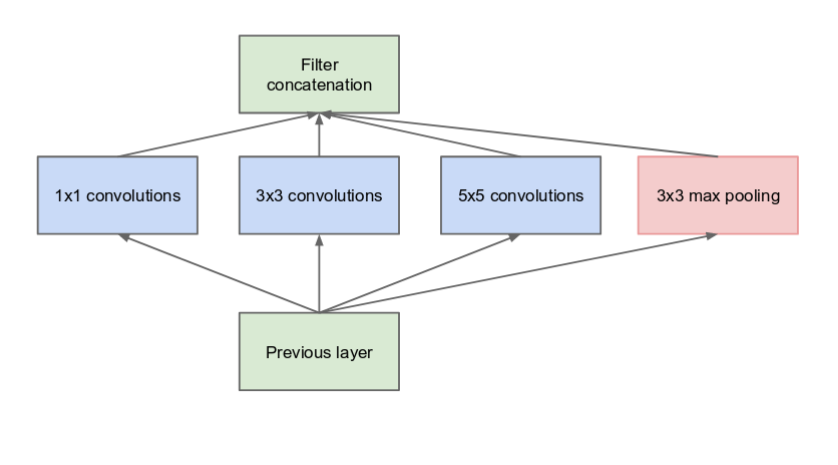
\includegraphics{plots/05_conv_variations/inception/incept_naive.png}}
    \caption{Naive inception module. The model can \enquote{choose} from kernels of different sizes.}
  \end{figure}
        \small{Idea: do several convolutions in parallel and concatenate the resulting feature maps in the depth dimension. This requires equal dimensions of the feature maps created by the parallel convolutions.Thus, same padding is used throughout the parallel convolutions.}
\framebreak 

    \begin{figure}
      \centering
      \scalebox{0.75}{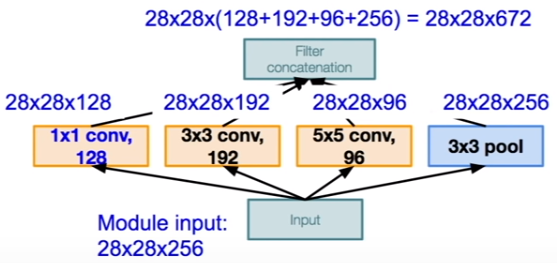
\includegraphics{plots/05_conv_variations/inception/incep_ex.png}}
      \tiny{\\ credit : Stanford University}
      \caption{\footnotesize{Naive Inception module - Example}}
      
    \end{figure}
    \begin{itemize}
        \item \small{To allow for the bypass of information throughout one inception module, an 1x1 convolutional layer is also included.
        \item Max-pooling is used as it is ought to increase the robustness of the feature maps. The kernels are padded accordingly to yield feature maps of equal dimensions.}
    \end{itemize}
\framebreak

    \begin{figure}
      \centering
      \scalebox{0.80}{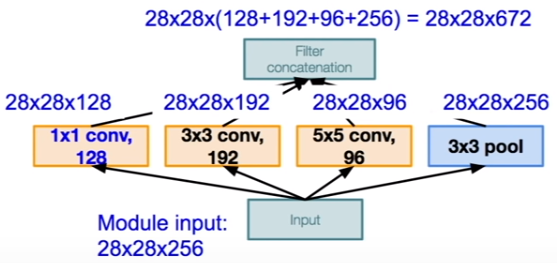
\includegraphics{plots/05_conv_variations/inception/incep_ex.png}}
      \tiny{\\ credit : Stanford University}
      \caption{\footnotesize{Naive Inception module - Example}}
    \end{figure}
    \begin{itemize}
        \item \small{Resulting feature map blocks are restricted to have the same dimensionality but can be of varying depth.
        \item The different feature maps are finally concatenated in the depth-dimension and fed to the next layer.}
    \end{itemize}
\framebreak

    \begin{figure}
        \centering
        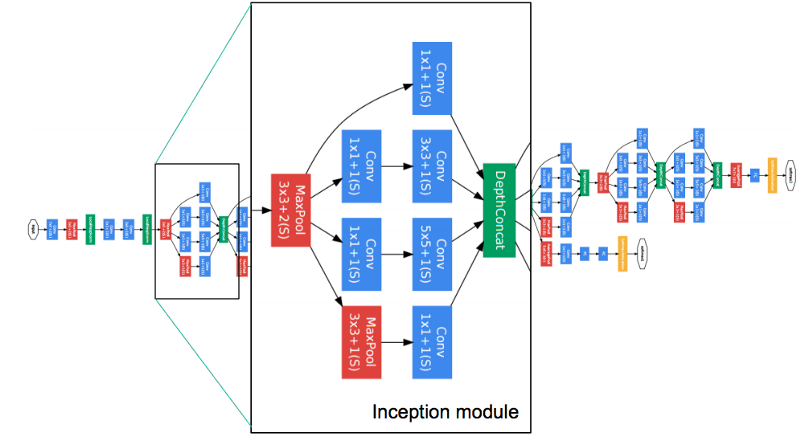
\includegraphics[width=11cm]{plots/05_conv_variations/inception/googlenet.png}
        \caption{Inception modules are the integral part of the famous GoogLeNet (2014), one of the first very deep net architectures.}
    \end{figure}
\end{vbframe}

%%%%%%%%%%%%%%%%%%%%%%%%%%%%%%%%%%%%%%%%%%%%%%%%%%%%%%%%%%%%%%%%%%
%%%%%%%%%%%%%%%%%%%%%%%%%%%%%%%%%%%%%%%%%%%%%%%%%%%%%%%%%%%%%%%%%%

\begin{vbframe}{Inception modules}
  \begin{figure}
    \centering
    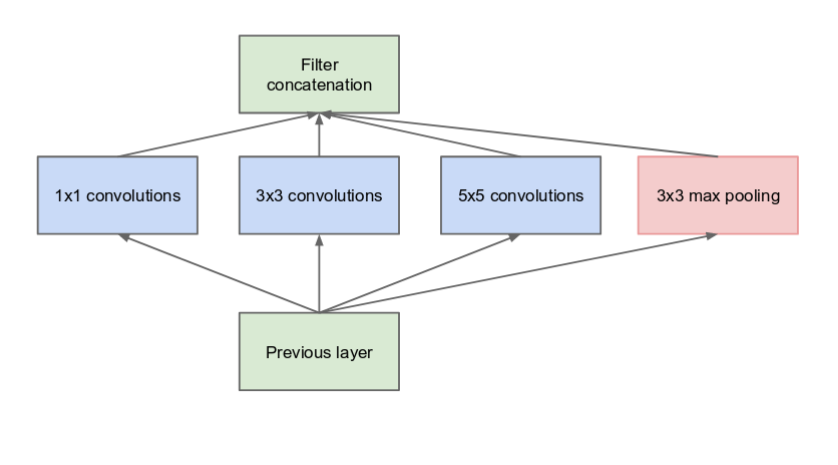
\includegraphics[width=8cm]{plots/05_conv_variations/inception/incept_naive.png}
    \caption{Naive inception module.}
  \end{figure}
    \begin{itemize}
        \item Problem: 3x3 and 5x5 convolutions are expensive operations, especially when executed on very deep input blocks such as many feature maps from the previous layer.
    \end{itemize}
\end{vbframe}


\begin{vbframe}{Inception modules}
  \begin{figure}
    \centering
    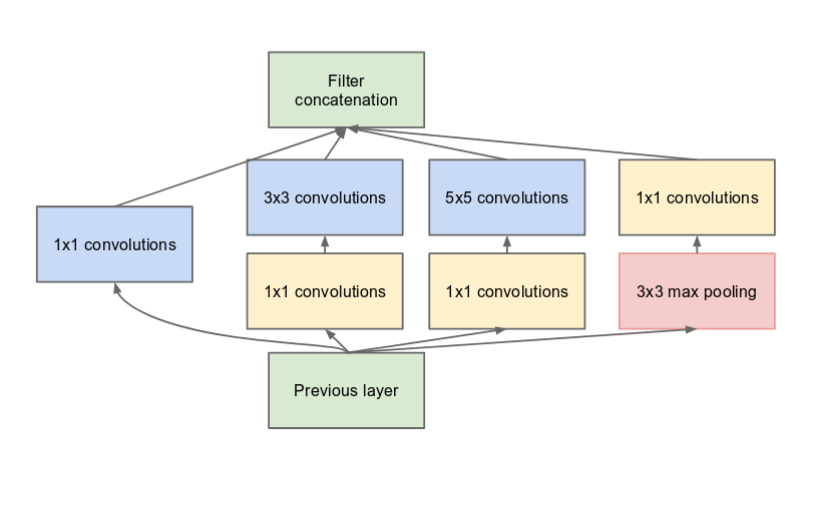
\includegraphics[width=8cm]{plots/05_conv_variations/inception/incept_dim_reduction.png}
    \caption{Dimensionality reduced inception module.}
  \end{figure}
    \begin{itemize}
        \item Solution: apply 1x1 convolutions beforehand to reduce the depth of the previous feature map.
    \end{itemize}
\end{vbframe}

\begin{vbframe}{Inception modules}
    \begin{itemize}
        \item Let us understand this with a little numerical example.
        \item Output dimensions of the previous layer: [28, 28, 192].
        \item Output dimensions of the 5x5 convolution from the inception module: [28, 28, 32].
        \item The 5x5 convolution has stride 1 and same padding.
        \item To improve speed, we first convolve the [28, 28, 192] input with 16 1x1 kernels which results in a [28, 28, 16] block. We then apply the 32 5x5 kernel convolution on this \enquote{thinner} block.
        \item Required operations:
        \begin{itemize}
            \item Naive: $5^2 \cdot 28^2 \cdot 192 \cdot 32 = 120.422.400$
            \item Improved version with 1x1 convolution and depth 16: $1^2 \cdot 28^2 \cdot 192 \cdot 16 + 5^2 \cdot 28^2 \cdot 16 \cdot 32 = 12.443.648$
        \end{itemize}
    \end{itemize}
\end{vbframe}



%%%%%%%%%%%%%%%%%%%%%%%%%%%%%%%%%%%%%%%%%%%%%%%%%%%%%%%%%%%%%%%%%%
%%%%%%%%%%%%%%%%%%%%%%%%%%%%%%%%%%%%%%%%%%%%%%%%%%%%%%%%%%%%%%%%%%


\section{Skip connections}

\begin{vbframe}{Skip connections}
    \begin{itemize}
        \item Problem setting: theoretically, we could build infinitely deep architectures as the net should learn to pick the beneficial layers and skip those that do not improve the performance automatically.
        \item But: this skipping would imply learning an identity mapping $\xv = \mathcal{F}(\xv)$. It is very hard for a neural net to learn such a 1:1 mapping through the many non-linear activations in the architecture.
        \item Solution: offer the model explicitly the opportunity to skip certain layers if they are not useful.
        \item Introduced in \textit{He et. al , 2015} and motivated by the observation that stacking evermore layers increases the test- as well as the train-error ($\neq$ overfitting).
    \end{itemize}
\framebreak

  \begin{figure}
    \centering
    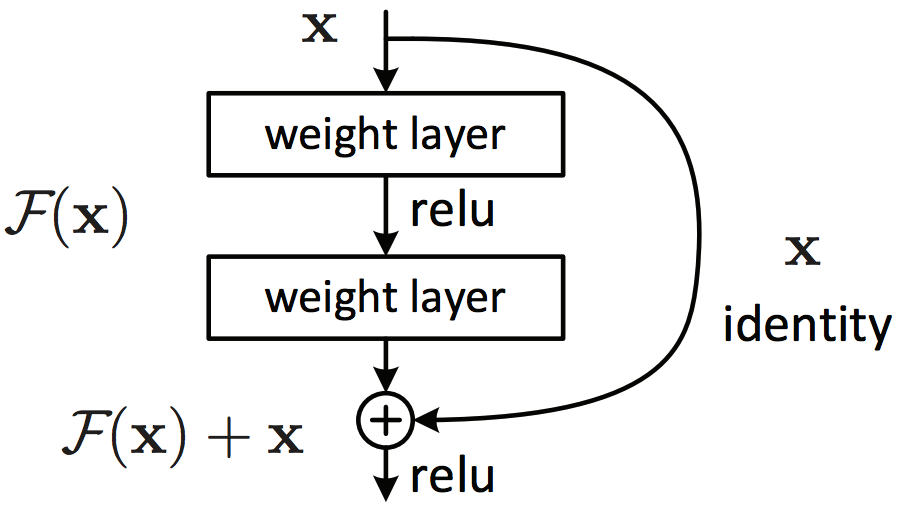
\includegraphics[width=7cm]{plots/05_conv_variations/skip/residual_module.png}
    \caption{Skip connection/ residual learning module. The information flows through two layers and the identity function. Both streams of information are then element-wise summed and jointly activated.}
  \end{figure}
\framebreak

    \begin{itemize}
        \item Let $\mathcal{H}(\xv)$ be the optimal underlying mapping that should be learned by (parts of) the net.
        \item $\xv$ is the input in layer $l$ (can be raw data input or the output of a previous layer).
        \item $\mathcal{H}(\xv)$ is the output from layer $l$.
        \item Instead of fitting $\mathcal{H}(\xv)$, the net is ought to learn the residual mapping $\mathcal{F}(\xv):=\mathcal{H}(\xv)-\xv$ whilst $\xv$ is added via the identity mapping.
        \item Thus, $\mathcal{H}(\xv) = \mathcal{F}(\xv) + \xv$, as formulated on the previous slide.
        \item The model should only learn the \textbf{residual mapping} $\mathcal{F}(\xv)$ 
        \item Thus, the procedure is also referred to as \textbf{Residual Learning}.
    \end{itemize}
\framebreak

    \begin{itemize}
        \item The element-wise addition of the learned residuals $\mathcal{F}(\xv)$ and the identity-mapped data $\xv$ requires both to have the same dimensions.
        \item To allow for downsampling within $\mathcal{F}(\xv)$ (via pooling or valid-padded convolutions), the authors introduce a linear projection layer $W_s$ .
        \item $W_s$ ensures that $\xv$ is brought to the same dimensionality as $\mathcal{F}(\xv)$ such that:
        $$
            y = \mathcal{F}(\xv) + W_s\xv,
        $$
        \item $y$ is the output of the skip module and $W_s$ represents the weight matrix of the linear projection (\# rows of $W_s$ = dimensionality of $\mathcal{F}(\xv)$).
        \item This idea applies to fully connected layers as well as to convolutional layers.
    \end{itemize}
\end{vbframe}


\section{Global average pooling}

\begin{vbframe}{Global average pooling}
    \begin{itemize}
        \item Problem setting: tackle overfitting in the final fully connected layer.
        \begin{itemize}
        \item Classic pooling removes spatial information and is mainly used for dimension and parameter reduction.
        \item The elements of the final feature maps are connected to the output layer via a dense layer. This could require a huge number of weights increasing the danger of overfitting.
        \item Example: 256 feature maps of dim 100x100 connected to 10 output neurons lead to $25.6\times 10^6$ weights for the final dense layer.
        \end{itemize}
        \framebreak 

        \item Solution: 
        \begin{itemize}
            \item Average each final feature map to the element of one global average pooling (GAP) vector.
            \item Do not use pooling throughout the net.
            \item Example: 256 feature maps are now reduced to GAP-vector of length 256 yielding a final dense layer with 2560 weights.
        \end{itemize}
    \end{itemize}

    \begin{figure}
        \centering
        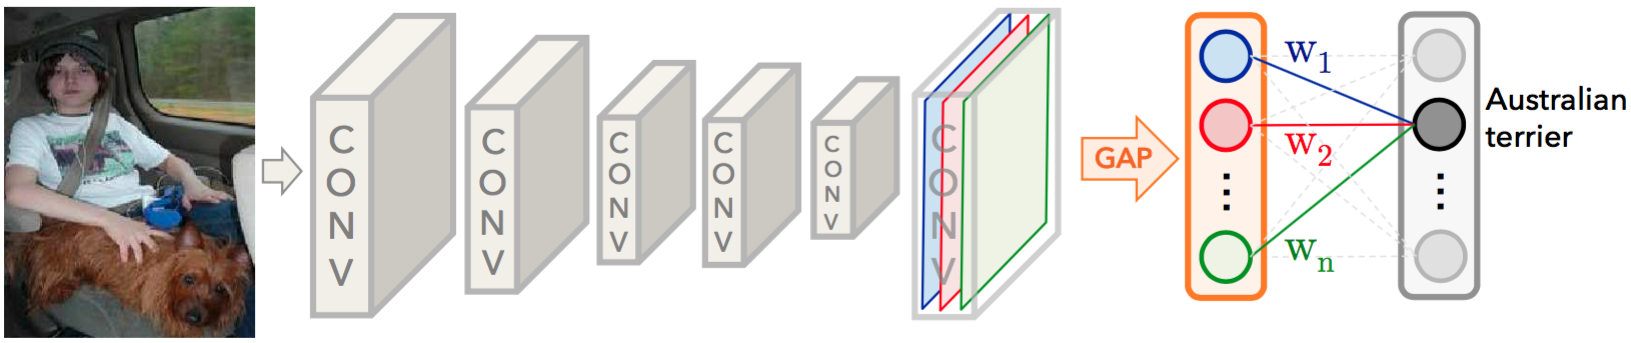
\includegraphics[width=11cm]{plots/05_conv_variations/gap/GAP.png}
        \small{\caption{Illustration of GAP. Each feature map representing one feature category averaged into one final vector. No pooling operations are applied throughout the net. The dimensionality of the input reduces solely due to the convolution operations. }}
    \end{figure}

\framebreak

    \begin{itemize}
        \item GAP preserves whole information from the single feature maps whilst decreasing the dimension.
        \item Mitigates the possibly \textbf{destructive} effect of pooling.
        \item Each element of the GAP output represents the activation of a certain feature on the input data.
        \item Acts as an additional regularizer on the final fully connected layer.
        \item Allows for interpretation of the model via Class Activation Maps (more on this later).
    \end{itemize}

\end{vbframe}


\begin{vbframe}{Class activation mapping}
    \begin{itemize}
        \item We want to understand the decision-making of a net, e.g. \textbf{why does it classify image X as a cat?}
        \item Simplest method based on GAP was introduced in \textit{Zhou et. al, 2016}.
        \item Idea: 
        \begin{itemize}
            \item the final GAP vector stores the activation of each feature map category that was learnt throughout the net.
            \item the dense layer that connects the output classes with the GAP vector stores information about how much each feature contributes to each class.
            \item exploit this information to show which parts of the input image would be activated for each class.
        \end{itemize}
    \end{itemize}
    
\framebreak

    \begin{figure}
    \centering
    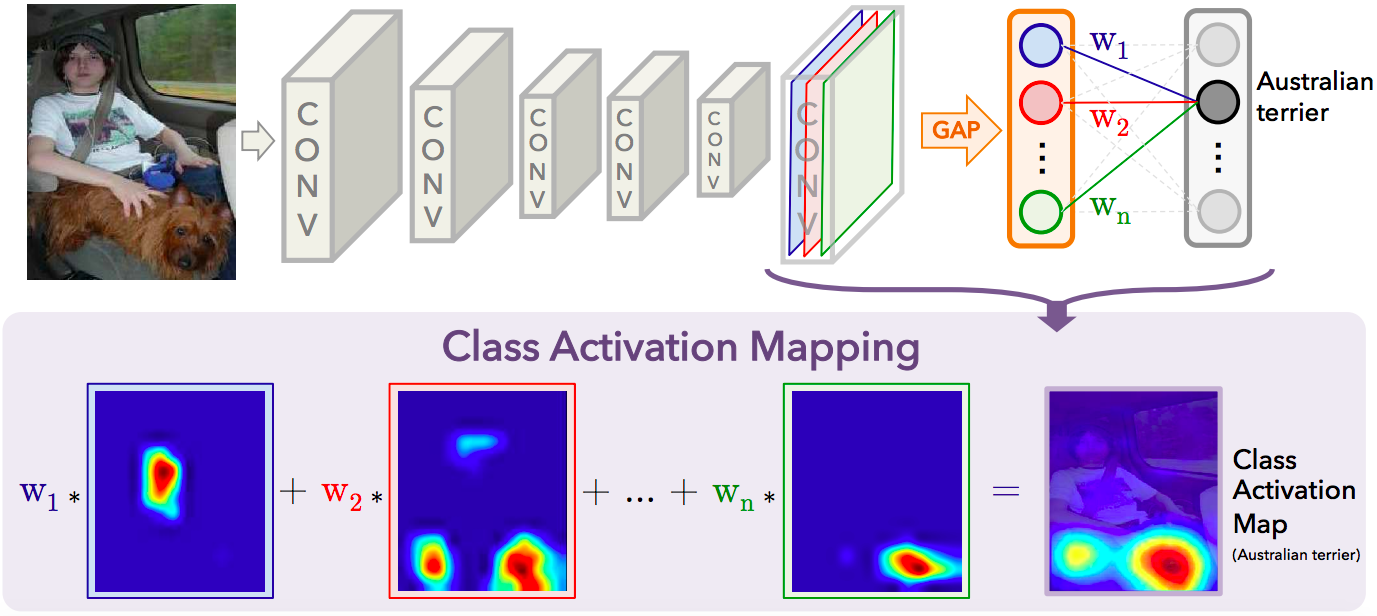
\includegraphics[width=11cm]{plots/05_conv_variations/cam/cam_scheme.png}
    \caption{Illustration of the class activation mapping. The activated regions from the feature maps are summed up weighted by their connection strength with the final output classes and upsampled back to the dimension of the input image. No max-pooling is applied throughout the architecture, the downsampling is due to the CNN layers. }
    \end{figure}
\framebreak

    \begin{enumerate}
        \item Train a net with GAP pooling end-to-end.
        \item Run a forward-pass with the image $i$ you would like to understand.
        \item Take the final $l$ feature maps $f_1, ..., f_l$ for this input.
        \item Get the \textit{feature weights} $w_{j1}, ...,w_{jl}$ that connect the GAP layer with the final class output $j$ that you would like to interpret (e.g. terrier).
        \item Create the \textbf{class activation map} (CAM) for class $j$ on input image $i$:
        $$
            \text{CAM}_{j, i} = \sum_{k = 1}^{l}w_{jk} * f_k
        $$
        \item Normalize the values such that $\text{CAM}_{j, i} \in [0, 1]$.
        \item In case of valid convolutions, the resulting CAM will be smaller than the input image. Linear upsampling is then used to map it back to the input dimension.
        \item Overlay the input image with the CAM and interpret the activation.
    \end{enumerate}

\end{vbframe}





%%%%%%%%%%%%%%%%%%%%%%%%%%%%%%%%%%%%%%%%%%%%%%%%%%%%%%%%%%%%%%%%%%
%%%%%%%%%%%%%%%%%%%%%%%%%%%%%%%%%%%%%%%%%%%%%%%%%%%%%%%%%%%%%%%%%%

%%%%%%%%%%%%%%%%%%%%%%%%%%%%%%%%%%%%%%%%%%%%%%%%%%%%%%%%%%%%%%%%%%
%%%%%%%%%%%%%%%%%%          REFERENCES          %%%%%%%%%%%%%%%%%%
%%%%%%%%%%%%%%%%%%%%%%%%%%%%%%%%%%%%%%%%%%%%%%%%%%%%%%%%%%%%%%%%%%
\begin{vbframe}
\frametitle{References}
\footnotesize{
\begin{thebibliography}{99}

% \bibitem[Ronneberger et al., 2015]{12} Olaf Ronneberger, Philipp Fischer, Thomas Brox (2015)
% \newblock U-Net: Convolutional Networks for Biomedical Image Segmentation
% \newblock \emph{\url{http://arxiv.org/abs/1505.04597}}
% %%%%%%%%%%%%%%%%%%%%%%%%%%%%%%%%%%
\bibitem[Zhou et. al , 2016]{25} B. Zhou, Khosla, A., Labedriza, A., Oliva, A. and A. Torralba (2016)
\newblock Deconvolution and Checkerboard Artifacts
\newblock \emph{\url{http://cnnlocalization.csail.mit.edu/Zhou_Learning_Deep_Features_CVPR_2016_paper.pdf}}
%%%%%%%%%%%%%%%%%%%%%%%%%%%%%%%%%%
%%%%%%%%%%%%%%%%%%%%%%%%%%%%%%%%%%
\bibitem[Szegedy et. al , 2014]{26} Christian Szegedy, Wei Liu, Yangqing Jia, Pierre Sermanet, Scott Reed, Dragomir Anguelov, Dumitru Erhan, Vincent Vanhoucke and Andrew Rabinovich (2014)
\newblock Going deeper with convolutions
\newblock \emph{\url{https://arxiv.org/abs/1409.4842}}
%%%%%%%%%%%%%%%%%%%%%%%%%%%%%%%%%%
%%%%%%%%%%%%%%%%%%%%%%%%%%%%%%%%%%
% \bibitem[Jie Hu et. al , 2014]{27} Jie Hu, Shen, Li and Gang Sun (2017)
% \newblock Squeeze-and-Excitation Networks
% \newblock \emph{\url{https://arxiv.org/abs/1709.01507}}
%%%%%%%%%%%%%%%%%%%%%%%%%%%%%%%%%%
%%%%%%%%%%%%%%%%%%%%%%%%%%%%%%%%%%
% \bibitem[Szegedy Christian et. al , 2015]{28} Christian Szegedy, Vanhoucke, Vincent, Sergey, Ioffe, Shlens, Jonathan and Wojna Zbigniew (2015)
% \newblock Rethinking the Inception Architecture for Computer Vision
% \newblock \emph{\url{https://arxiv.org/abs/1512.00567}}
%%%%%%%%%%%%%%%%%%%%%%%%%%%%%%%%%%
%%%%%%%%%%%%%%%%%%%%%%%%%%%%%%%%%%
\bibitem[He et. al , 2015]{29} Kaiming He, Zhang, Xiangyu, Ren, Shaoqing, and Jian Sun (2015)
\newblock Deep Residual Learning for Image Recognition
\newblock \emph{\url{https://arxiv.org/abs/1512.03385}}
%%%%%%%%%%%%%%%%%%%%%%%%%%%%%%%%%%
%%%%%%%%%%%%%%%%%%%%%%%%%%%%%%%%%%
\bibitem[Zhou et. al, 2016]{32} Bolei Zhou, Aditya Khosla, Agata Lapedriza, Aude Oliva and Antonio Torralba (2016)
\newblock Learning Deep Features for Discriminative Localization
\newblock \emph{\url{http://cnnlocalization.csail.mit.edu/Zhou_Learning_Deep_Features_CVPR_2016_paper.pdf}}
%%%%%%%%%%%%%%%%%%%%%%%%%%%%%%%%%%
%%%%%%%%%%%%%%%%%%%%%%%%%%%%%%%%%%



\end{thebibliography}
}
\end{vbframe}

%%%%%%%%%%%%%%%%%%%%%%%%%%%%%%%%%%%%%%%%%%%%%%%%%%%%%%%%%%%%%%%%%%
%%%%%%%%%%%%%%%%%%%%%%%%%%%%%%%%%%%%%%%%%%%%%%%%%%%%%%%%%%%%%%%%%%
\endlecture
\end{document}
